\appendix
\chapter{Experimental Data}
\label{app:experimental_data}

\section{Experiment 1}
\label{app_sec:experiment_1}

\subsection{Support Vector Machine}
\label{app_sub:experiment_1_svm}
% params: test_1, svm

% Figure for \gls{swr} for acra using \gls{svm}
\begin{figure}
\centering
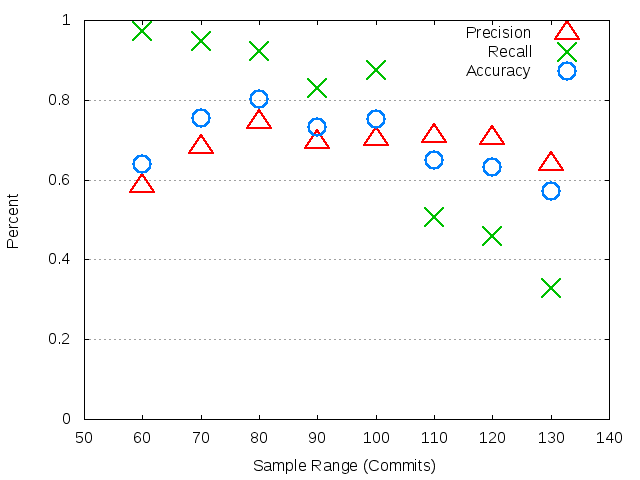
\includegraphics[width=0.8\textwidth]{images/svm/test_1/acra_sample_range.png}
\caption{\gls{swr} for acra using \gls{svm}}
\label{fig:test_1_acra_svm}
\end{figure}


% Figure for \gls{swr} for yardstick using \gls{svm}
\begin{figure}
\centering
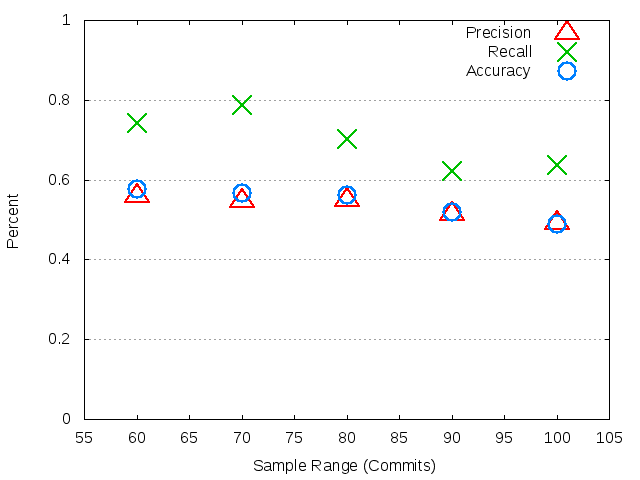
\includegraphics[width=0.8\textwidth]{images/svm/test_1/yardstick_sample_range.png}
\caption{\gls{swr} for yardstick using \gls{svm}}
\label{fig:test_1_yardstick_svm}
\end{figure}

\clearpage

% Figure for \gls{swr} for cardslib using \gls{svm}
\begin{figure}[!t]
\centering
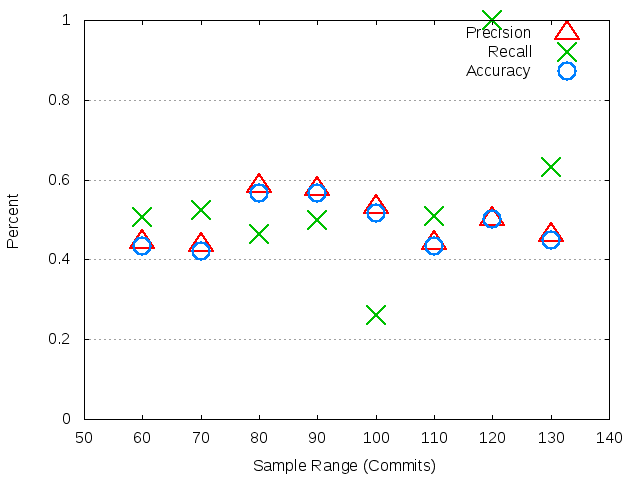
\includegraphics[width=0.8\textwidth]{images/svm/test_1/cardslib_sample_range.png}
\caption{\gls{swr} for cardslib using \gls{svm}}
\label{fig:test_1_cardslib_svm}
\end{figure}

% Figure for \gls{swr} for greenDAO using \gls{svm}
\begin{figure}[!t]
\centering
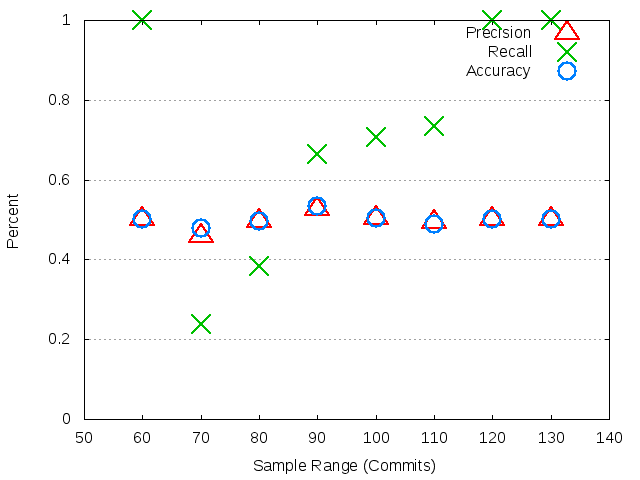
\includegraphics[width=0.8\textwidth]{images/svm/test_1/greenDAO_sample_range.png}
\caption{\gls{swr} for greenDAO using \gls{svm}}
\label{fig:test_1_greenDAO_svm}
\end{figure}

% Figure for \gls{swr} for mapstruct using \gls{svm}
\begin{figure}[!t]
\centering
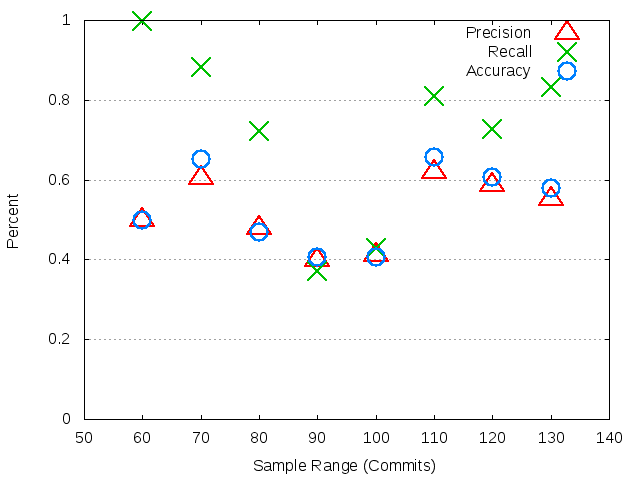
\includegraphics[width=0.8\textwidth]{images/svm/test_1/mapstruct_sample_range.png}
\caption{\gls{swr} for mapstruct using \gls{svm}}
\label{fig:test_1_mapstruct_svm}
\end{figure}

% Figure for \gls{swr} for deeplearning4j using \gls{svm}
\begin{figure}[!t]
\centering
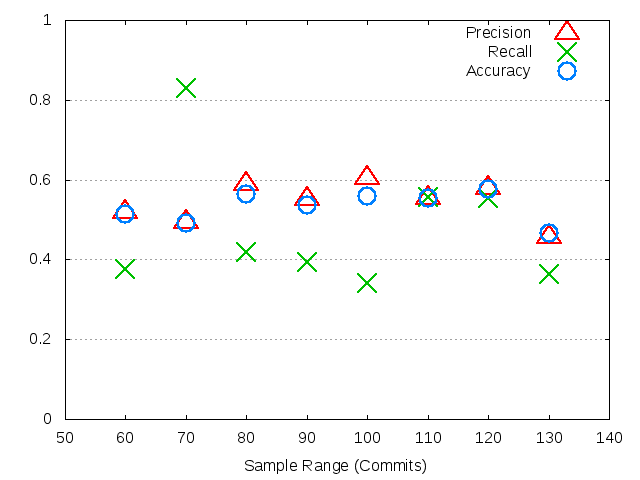
\includegraphics[width=0.8\textwidth]{images/svm/test_1/deeplearning4j_sample_range.png}
\caption{\gls{swr} for deeplearning4j using \gls{svm}}
\label{fig:test_1_deeplearning4j_svm}
\end{figure}

% Figure for \gls{swr} for governator using \gls{svm}
\begin{figure}[!t]
\centering
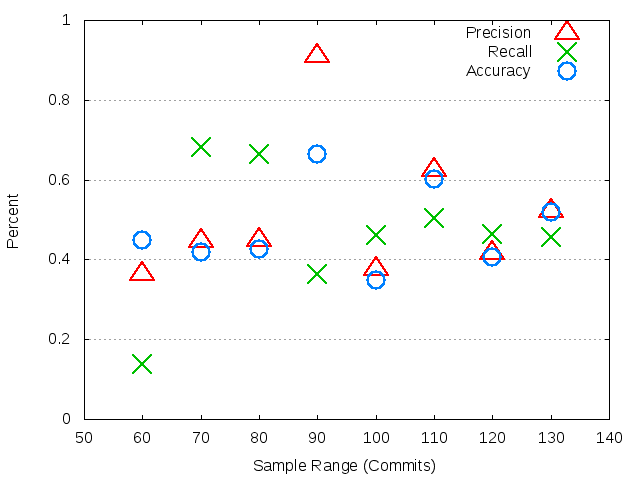
\includegraphics[width=0.8\textwidth]{images/svm/test_1/governator_sample_range.png}
\caption{\gls{swr} for governator using \gls{svm}}
\label{fig:test_1_governator_svm}
\end{figure}

% Figure for \gls{swr} for arquillian-core using \gls{svm}
\begin{figure}[!t]
\centering
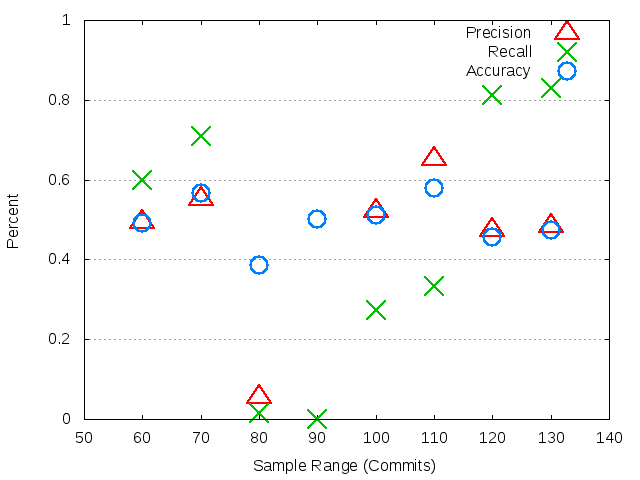
\includegraphics[width=0.8\textwidth]{images/svm/test_1/arquillian-core_sample_range.png}
\caption{\gls{swr} for arquillian-core using \gls{svm}}
\label{fig:test_1_arquillian-core_svm}
\end{figure}

% Figure for \gls{swr} for fresco using \gls{svm}
\begin{figure}[!t]
\centering
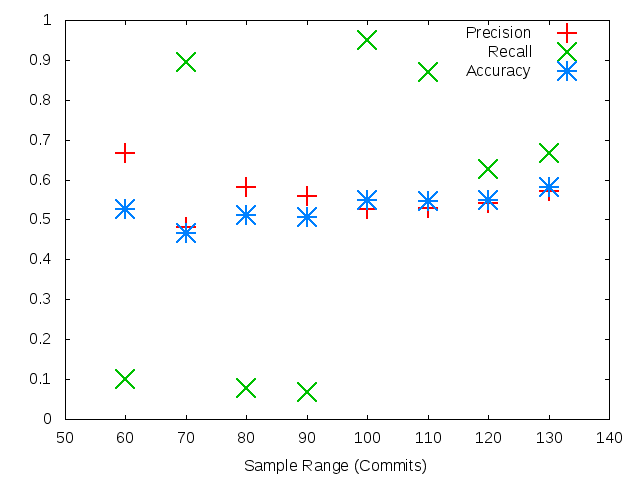
\includegraphics[width=0.8\textwidth]{images/svm/test_1/fresco_sample_range.png}
\caption{\gls{swr} for fresco using \gls{svm}}
\label{fig:test_1_fresco_svm}
\end{figure}

% Figure for \gls{swr} for jadx using \gls{svm}
\begin{figure}[!t]
\centering
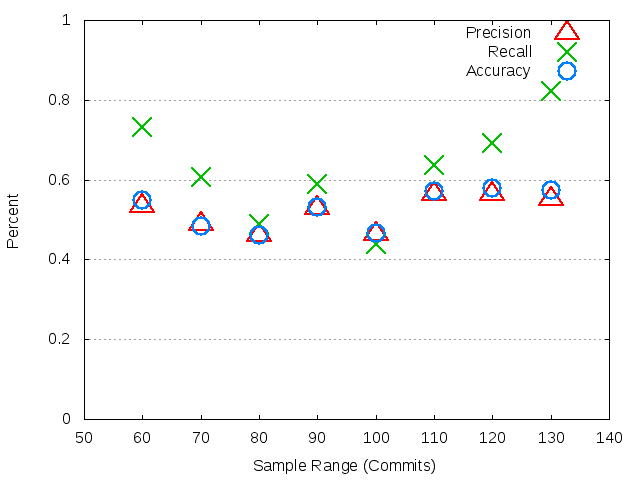
\includegraphics[width=0.8\textwidth]{images/svm/test_1/jadx_sample_range.png}
\caption{\gls{swr} for jadx using \gls{svm}}
\label{fig:test_1_jadx_svm}
\end{figure}

% Figure for \gls{swr} for nettosphere using \gls{svm}
\begin{figure}[!t]
\centering
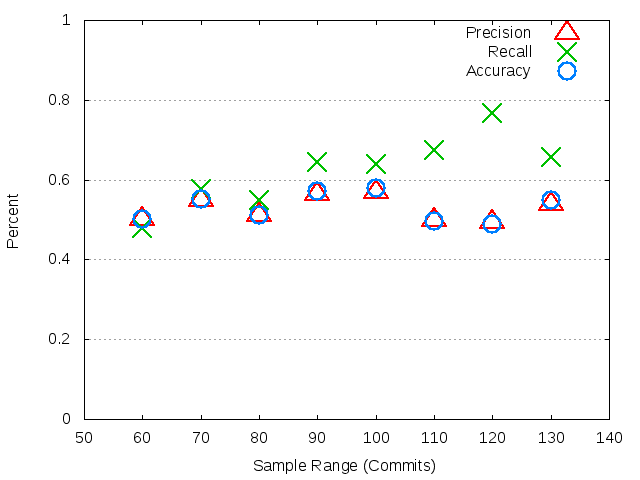
\includegraphics[width=0.8\textwidth]{images/svm/test_1/nettosphere_sample_range.png}
\caption{\gls{swr} for nettosphere using \gls{svm}}
\label{fig:test_1_nettosphere_svm}
\end{figure}

\clearpage
% Figure for \gls{swr} for storm using \gls{svm}
\begin{figure}[!t]
\centering
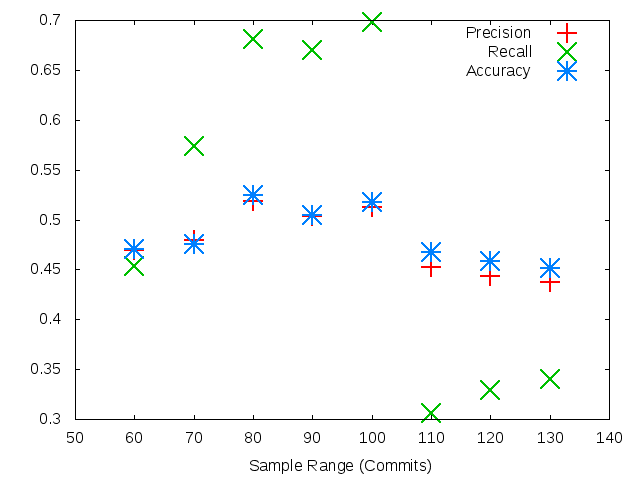
\includegraphics[width=0.8\textwidth]{images/svm/test_1/storm_sample_range.png}
\caption{\gls{swr} for storm using \gls{svm}}
\label{fig:test_1_storm_svm}
\end{figure}

% Figure for \gls{swr} for smile using \gls{svm}
\begin{figure}[!t]
\centering
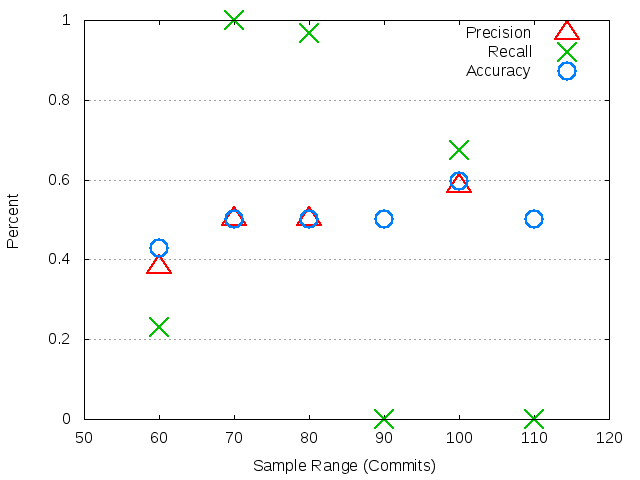
\includegraphics[width=0.8\textwidth]{images/svm/test_1/smile_sample_range.png}
\caption{\gls{swr} for smile using \gls{svm}}
\label{fig:test_1_smile_svm}
\end{figure}

% Figure for \gls{swr} for ShowcaseView using \gls{svm}
\begin{figure}[!t]
\centering
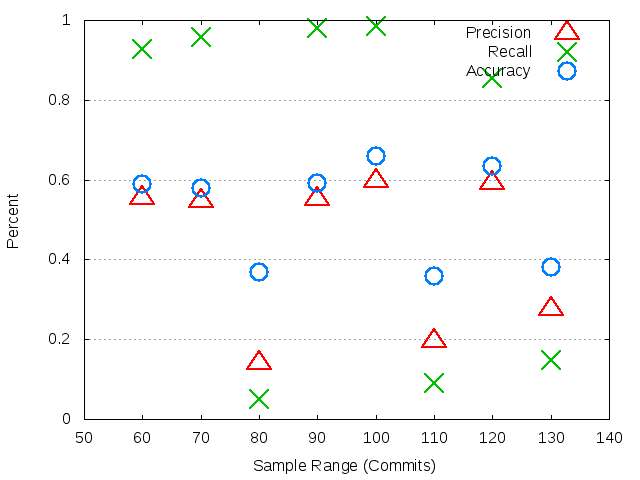
\includegraphics[width=0.8\textwidth]{images/svm/test_1/ShowcaseView_sample_range.png}
\caption{\gls{swr} for ShowcaseView using \gls{svm}}
\label{fig:test_1_ShowcaseView_svm}
\end{figure}

% Figure for \gls{swr} for tempto using \gls{svm}
\begin{figure}[!t]
\centering
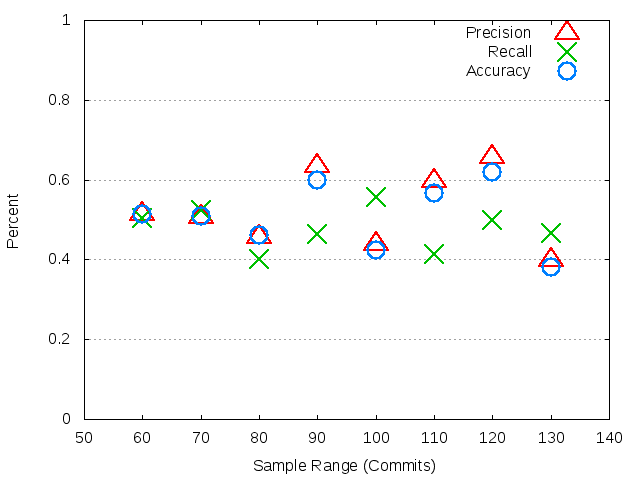
\includegraphics[width=0.8\textwidth]{images/svm/test_1/tempto_sample_range.png}
\caption{\gls{swr} for tempto using \gls{svm}}
\label{fig:test_1_tempto_svm}
\end{figure}

% Figure for \gls{swr} for retrolambda using \gls{svm}
\begin{figure}[!t]
\centering
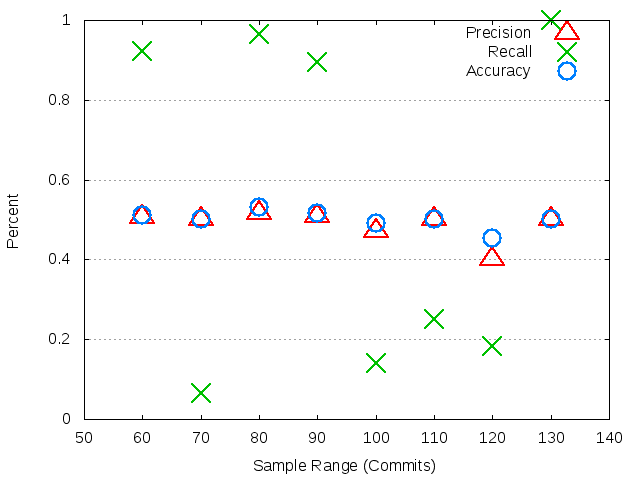
\includegraphics[width=0.8\textwidth]{images/svm/test_1/retrolambda_sample_range.png}
\caption{\gls{swr} for retrolambda using \gls{svm}}
\label{fig:test_1_retrolambda_svm}
\end{figure}

% Figure for \gls{swr} for blockly-android using \gls{svm}
\begin{figure}[!t]
\centering
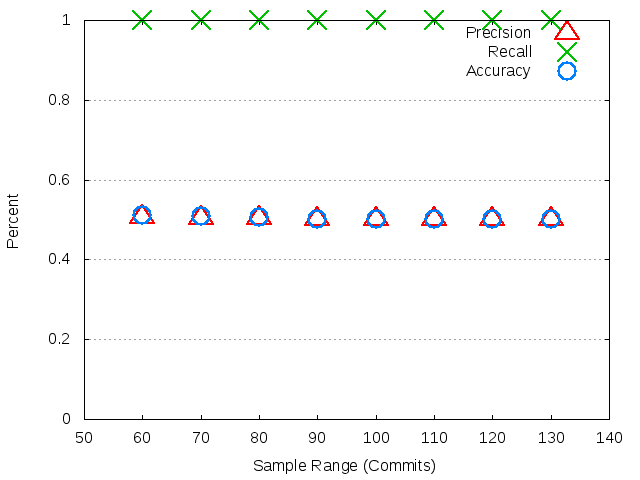
\includegraphics[width=0.8\textwidth]{images/svm/test_1/blockly-android_sample_range.png}
\caption{\gls{swr} for blockly-android using \gls{svm}}
\label{fig:test_1_blockly-android_svm}
\end{figure}

% Figure for \gls{swr} for ion using \gls{svm}
\begin{figure}[!t]
\centering
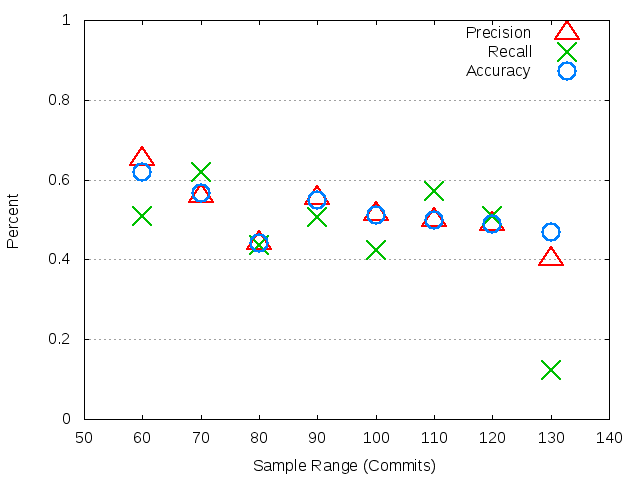
\includegraphics[width=0.8\textwidth]{images/svm/test_1/ion_sample_range.png}
\caption{\gls{swr} for ion using \gls{svm}}
\label{fig:test_1_ion_svm}
\end{figure}

% Figure for \gls{swr} for brave using \gls{svm}
\begin{figure}[!t]
\centering
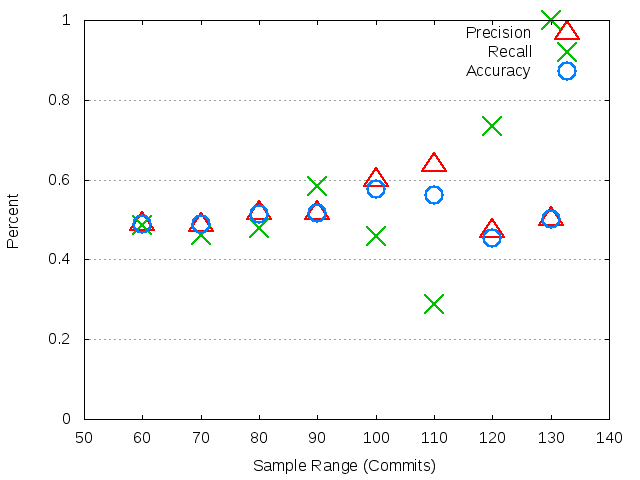
\includegraphics[width=0.8\textwidth]{images/svm/test_1/brave_sample_range.png}
\caption{\gls{swr} for brave using \gls{svm}}
\label{fig:test_1_brave_svm}
\end{figure}

% Figure for \gls{swr} for dagger using \gls{svm}
\begin{figure}[!t]
\centering
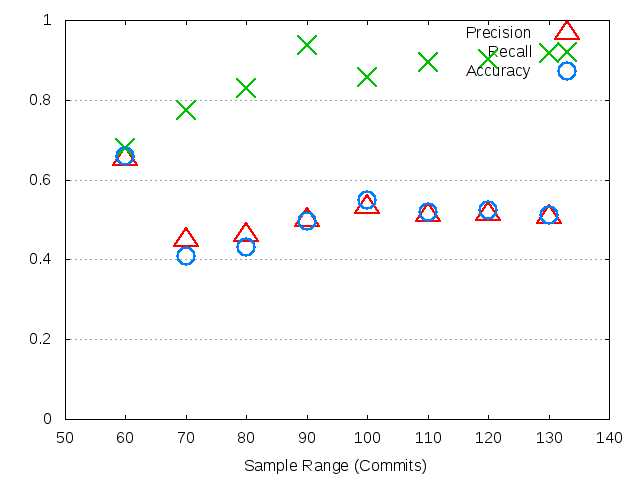
\includegraphics[width=0.8\textwidth]{images/svm/test_1/dagger_sample_range.png}
\caption{\gls{swr} for dagger using \gls{svm}}
\label{fig:test_1_dagger_svm}
\end{figure}

% Figure for \gls{swr} for parceler using \gls{svm}
\begin{figure}[!t]
\centering
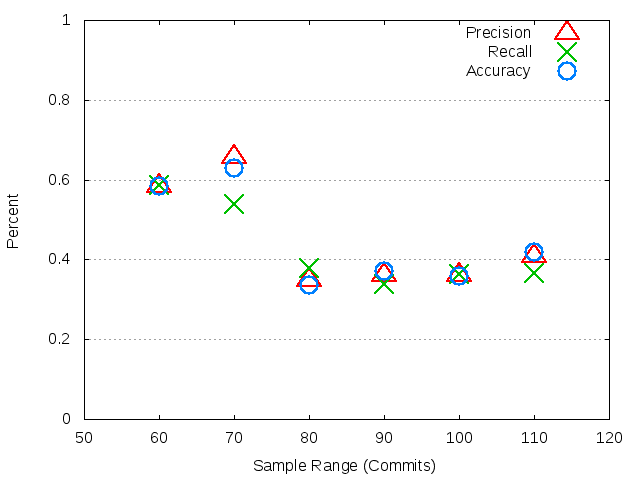
\includegraphics[width=0.8\textwidth]{images/svm/test_1/parceler_sample_range.png}
\caption{\gls{swr} for parceler using \gls{svm}}
\label{fig:test_1_parceler_svm}
\end{figure}

\clearpage
% Figure for \gls{swr} for spark using \gls{svm}
\begin{figure}[!t]
\centering
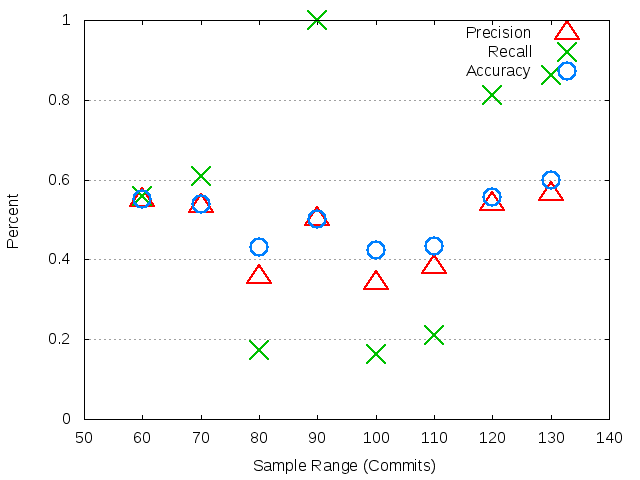
\includegraphics[width=0.8\textwidth]{images/svm/test_1/spark_sample_range.png}
\caption{\gls{swr} for spark using \gls{svm}}
\label{fig:test_1_spark_svm}
\end{figure}

% Figure for \gls{swr} for http-request using \gls{svm}
\begin{figure}[!t]
\centering
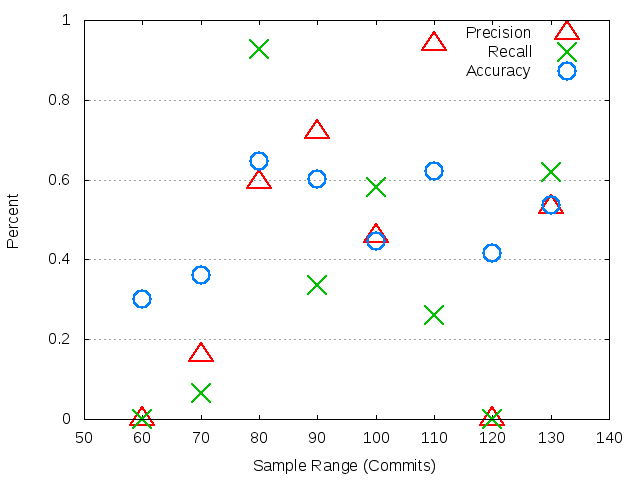
\includegraphics[width=0.8\textwidth]{images/svm/test_1/http-request_sample_range.png}
\caption{\gls{swr} for http-request using \gls{svm}}
\label{fig:test_1_http-request_svm}
\end{figure}

\subsection{Random Forest}
\label{app_sub:experiment_1_rf}
% params: test_1, rf
% has importance diagrams because it is random forest

% Figure for \gls{swr} for acra using \gls{rf}
\begin{figure}[!t]
\centering
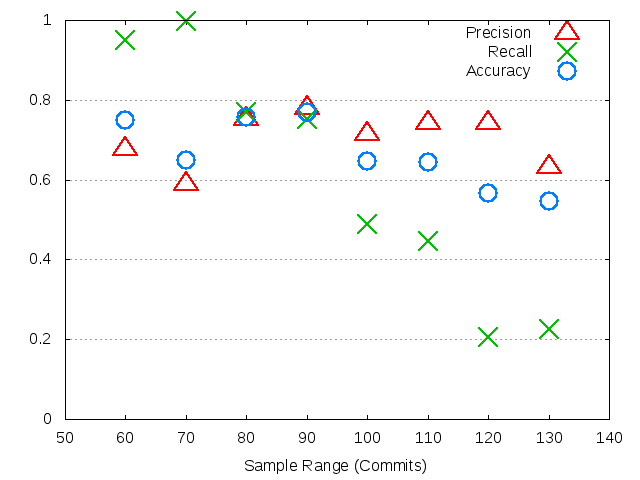
\includegraphics[width=0.8\textwidth]{images/rf/test_1/acra_sample_range.png}
\caption{\gls{swr} for acra using \gls{rf}}
\label{fig:test_1_acra_rf}
\end{figure}

\clearpage
% Figure for \gls{swr} for yardstick using \gls{rf}
\begin{figure}[!t]
\centering
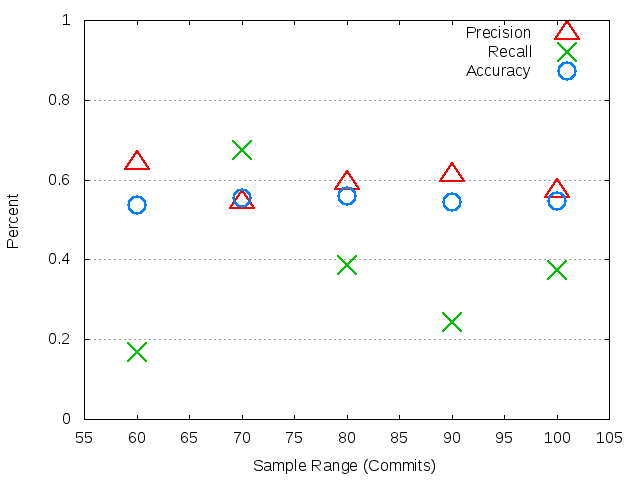
\includegraphics[width=0.8\textwidth]{images/rf/test_1/yardstick_sample_range.png}
\caption{\gls{swr} for yardstick using \gls{rf}}
\label{fig:test_1_yardstick_rf}
\end{figure}

% Figure for Feature Importance \gls{swr} for yardstick using \gls{rf}
\begin{figure}[!t]
\centering
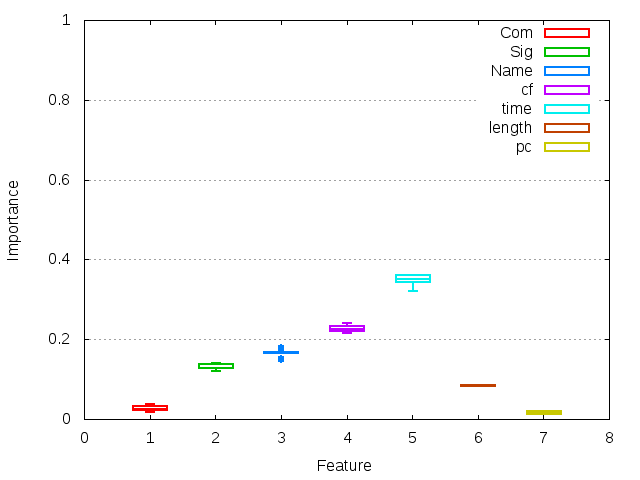
\includegraphics[width=0.8\textwidth]{images/rf/test_1/yardstick_importance.png}
\caption{Feature Importance \gls{swr} for yardstick using \gls{rf}}
\label{fig:test_1_yardstick_rf_importance}
\end{figure}

% Figure for \gls{swr} for cardslib using \gls{rf}
\begin{figure}[!t]
\centering
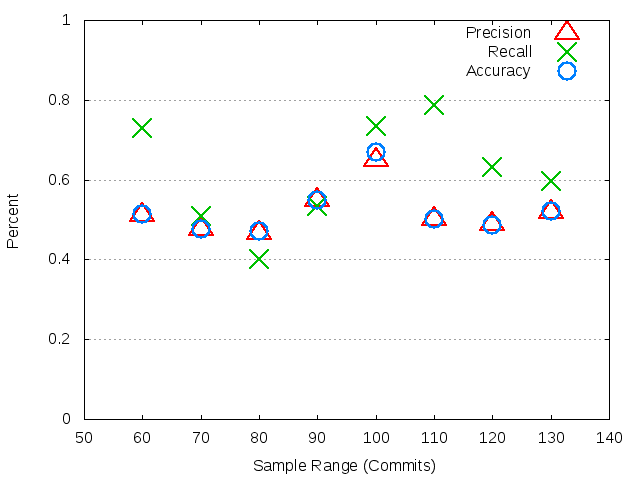
\includegraphics[width=0.8\textwidth]{images/rf/test_1/cardslib_sample_range.png}
\caption{\gls{swr} for cardslib using \gls{rf}}
\label{fig:test_1_cardslib_rf}
\end{figure}

% Figure for Feature Importance \gls{swr} for cardslib using \gls{rf}
\begin{figure}[!t]
\centering
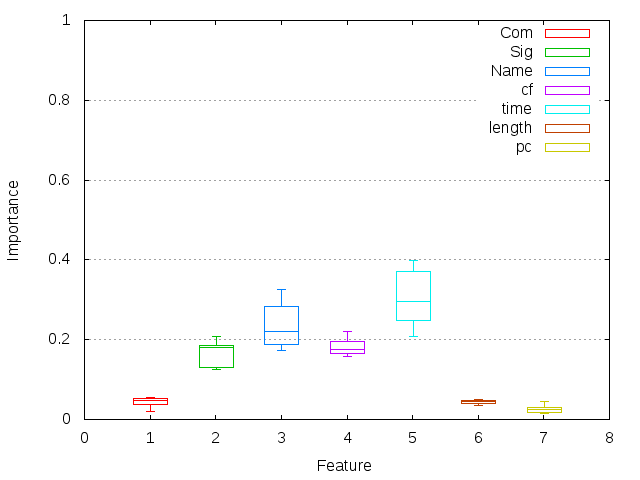
\includegraphics[width=0.8\textwidth]{images/rf/test_1/cardslib_importance.png}
\caption{Feature Importance \gls{swr} for cardslib using \gls{rf}}
\label{fig:test_1_cardslib_rf_importance}
\end{figure}

% Figure for \gls{swr} for greenDAO using \gls{rf}
\begin{figure}[!t]
\centering
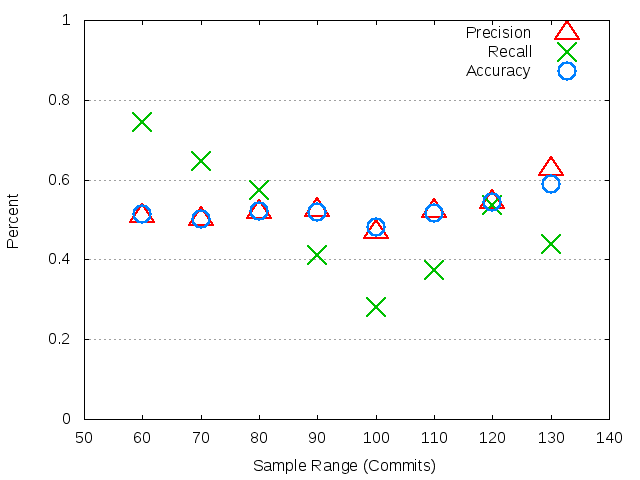
\includegraphics[width=0.8\textwidth]{images/rf/test_1/greenDAO_sample_range.png}
\caption{\gls{swr} for greenDAO using \gls{rf}}
\label{fig:test_1_greenDAO_rf}
\end{figure}

% Figure for Feature Importance \gls{swr} for greenDAO using \gls{rf}
\begin{figure}[!t]
\centering
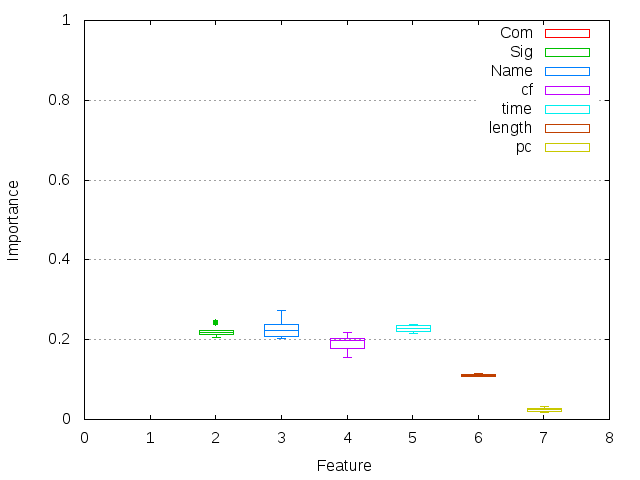
\includegraphics[width=0.8\textwidth]{images/rf/test_1/greenDAO_importance.png}
\caption{Feature Importance \gls{swr} for greenDAO using \gls{rf}}
\label{fig:test_1_greenDAO_rf_importance}
\end{figure}

% Figure for \gls{swr} for mapstruct using \gls{rf}
\begin{figure}[!t]
\centering
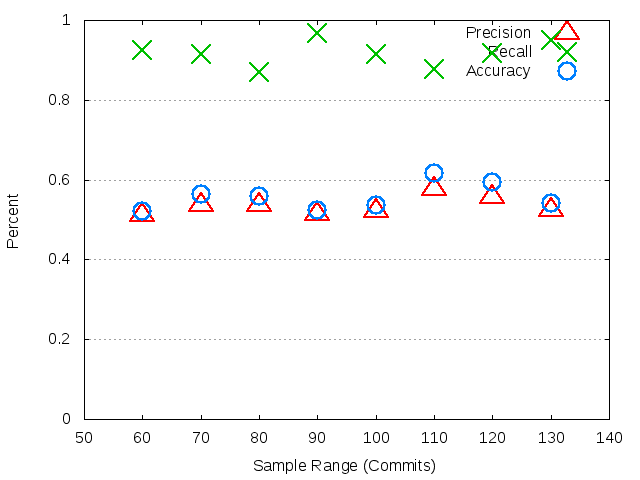
\includegraphics[width=0.8\textwidth]{images/rf/test_1/mapstruct_sample_range.png}
\caption{\gls{swr} for mapstruct using \gls{rf}}
\label{fig:test_1_mapstruct_rf}
\end{figure}

% Figure for Feature Importance \gls{swr} for mapstruct using \gls{rf}
\begin{figure}[!t]
\centering
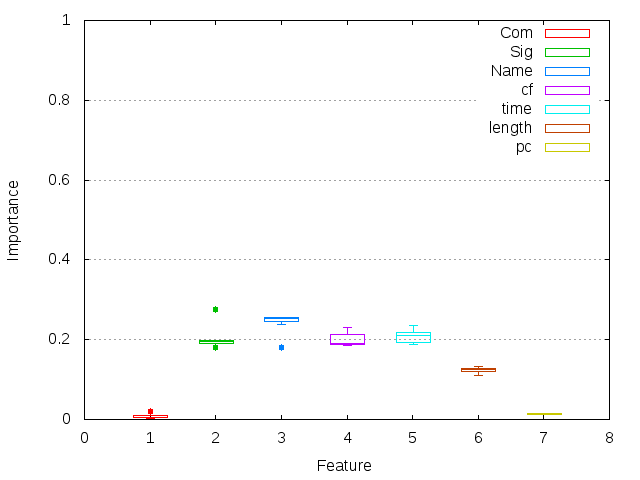
\includegraphics[width=0.8\textwidth]{images/rf/test_1/mapstruct_importance.png}
\caption{Feature Importance \gls{swr} for mapstruct using \gls{rf}}
\label{fig:test_1_mapstruct_rf_importance}
\end{figure}

% Figure for \gls{swr} for deeplearning4j using \gls{rf}
\begin{figure}[!t]
\centering
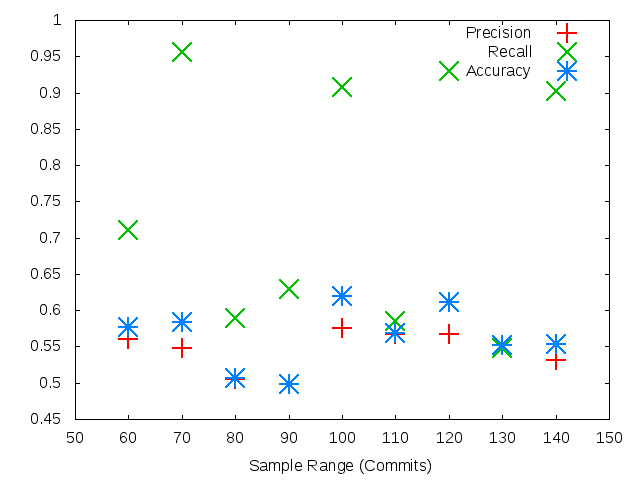
\includegraphics[width=0.8\textwidth]{images/rf/test_1/deeplearning4j_sample_range.png}
\caption{\gls{swr} for deeplearning4j using \gls{rf}}
\label{fig:test_1_deeplearning4j_rf}
\end{figure}

% Figure for \gls{swr} for governator using \gls{rf}
\begin{figure}[!t]
\centering
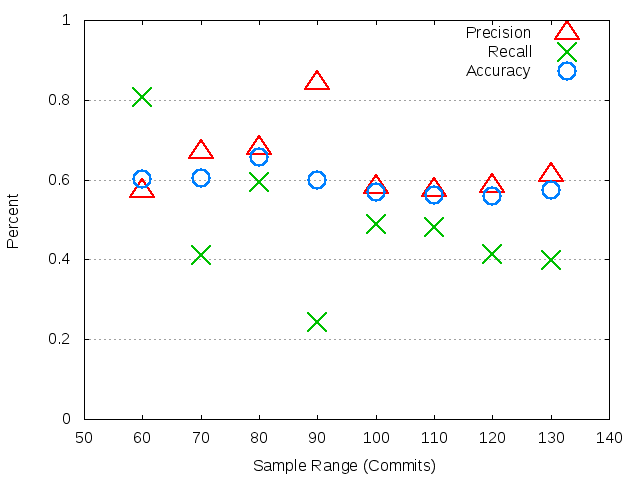
\includegraphics[width=0.8\textwidth]{images/rf/test_1/governator_sample_range.png}
\caption{\gls{swr} for governator using \gls{rf}}
\label{fig:test_1_governator_rf}
\end{figure}

% Figure for Feature Importance \gls{swr} for governator using \gls{rf}
\begin{figure}[!t]
\centering
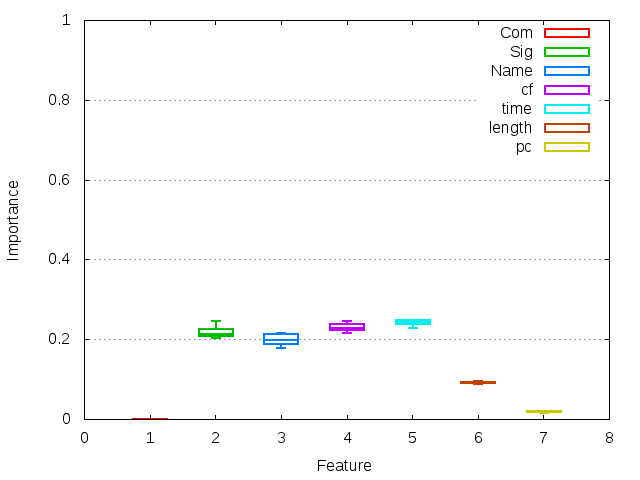
\includegraphics[width=0.8\textwidth]{images/rf/test_1/governator_importance.png}
\caption{Feature Importance \gls{swr} for governator using \gls{rf}}
\label{fig:test_1_governator_rf_importance}
\end{figure}

% Figure for \gls{swr} for arquillian-core using \gls{rf}
\begin{figure}[!t]
\centering
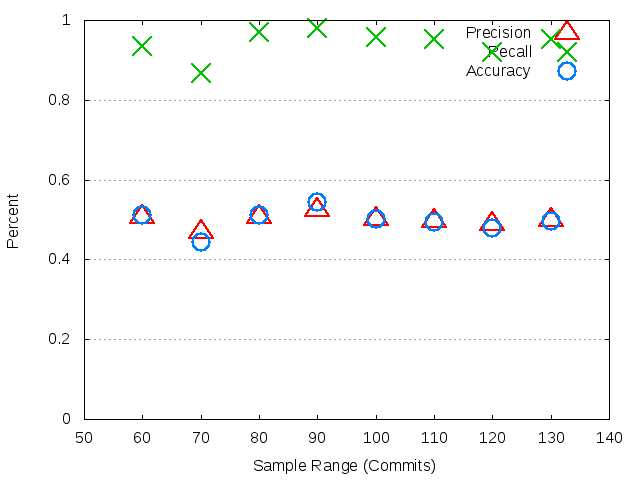
\includegraphics[width=0.8\textwidth]{images/rf/test_1/arquillian-core_sample_range.png}
\caption{\gls{swr} for arquillian-core using \gls{rf}}
\label{fig:test_1_arquillian-core_rf}
\end{figure}

% Figure for Feature Importance \gls{swr} for arquillian-core using \gls{rf}
\begin{figure}[!t]
\centering
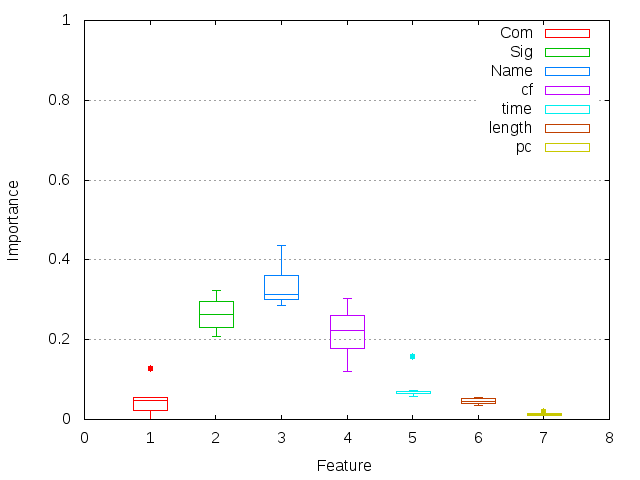
\includegraphics[width=0.8\textwidth]{images/rf/test_1/arquillian-core_importance.png}
\caption{Feature Importance \gls{swr} for arquillian-core using \gls{rf}}
\label{fig:test_1_arquillian-core_rf_importance}
\end{figure}

% Figure for \gls{swr} for fresco using \gls{rf}
\begin{figure}[!t]
\centering
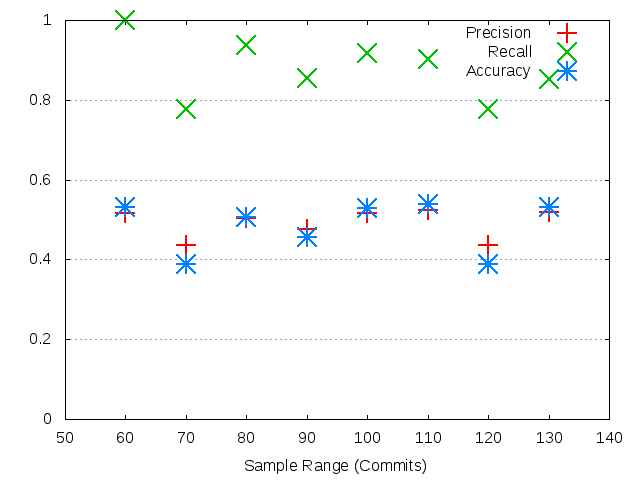
\includegraphics[width=0.8\textwidth]{images/rf/test_1/fresco_sample_range.png}
\caption{\gls{swr} for fresco using \gls{rf}}
\label{fig:test_1_fresco_rf}
\end{figure}

% Figure for \gls{swr} for jadx using \gls{rf}
\begin{figure}[!t]
\centering
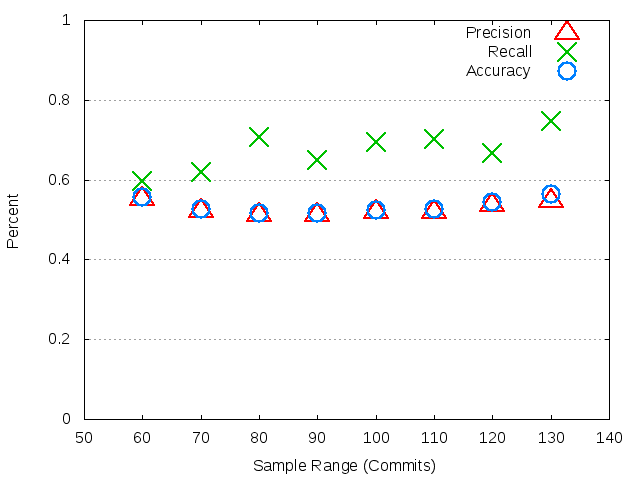
\includegraphics[width=0.8\textwidth]{images/rf/test_1/jadx_sample_range.png}
\caption{\gls{swr} for jadx using \gls{rf}}
\label{fig:test_1_jadx_rf}
\end{figure}

% Figure for Feature Importance \gls{swr} for jadx using \gls{rf}
\begin{figure}[!t]
\centering
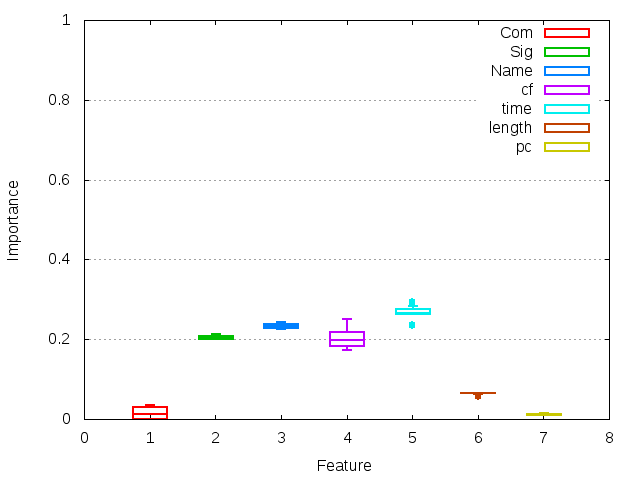
\includegraphics[width=0.8\textwidth]{images/rf/test_1/jadx_importance.png}
\caption{Feature Importance \gls{swr} for jadx using \gls{rf}}
\label{fig:test_1_jadx_rf_importance}
\end{figure}

% Figure for \gls{swr} for nettosphere using \gls{rf}
\begin{figure}[!t]
\centering
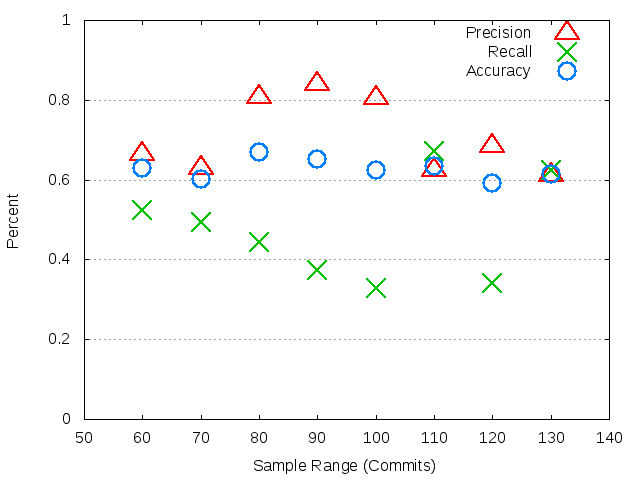
\includegraphics[width=0.8\textwidth]{images/rf/test_1/nettosphere_sample_range.png}
\caption{\gls{swr} for nettosphere using \gls{rf}}
\label{fig:test_1_nettosphere_rf}
\end{figure}

% Figure for Feature Importance \gls{swr} for nettosphere using \gls{rf}
\begin{figure}[!t]
\centering
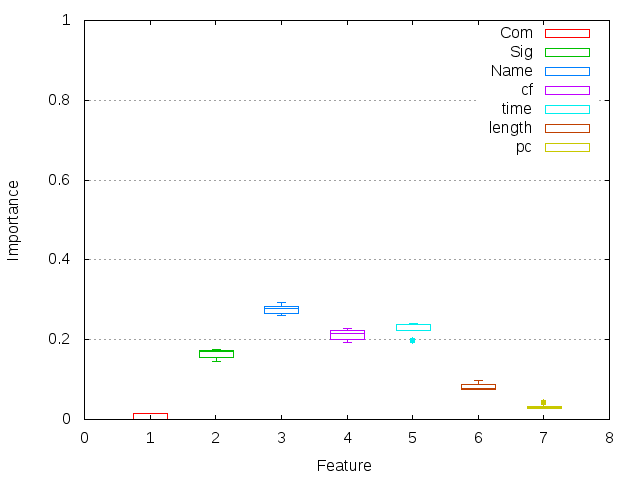
\includegraphics[width=0.8\textwidth]{images/rf/test_1/nettosphere_importance.png}
\caption{Feature Importance \gls{swr} for nettosphere using \gls{rf}}
\label{fig:test_1_nettosphere_rf_importance}
\end{figure}

\clearpage
% Figure for \gls{swr} for storm using \gls{rf}
\begin{figure}[!t]
\centering
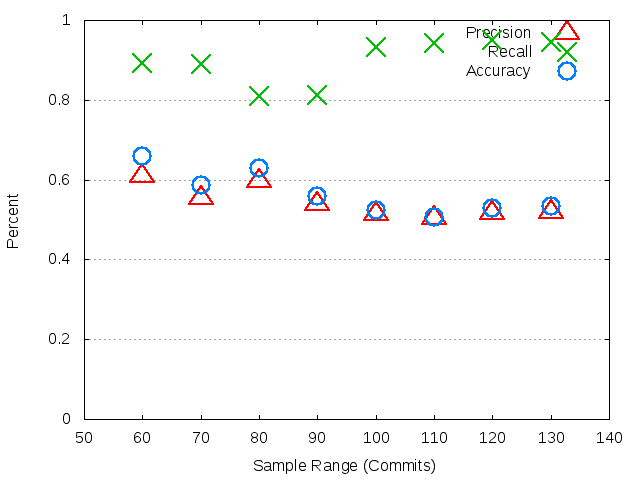
\includegraphics[width=0.8\textwidth]{images/rf/test_1/storm_sample_range.png}
\caption{\gls{swr} for storm using \gls{rf}}
\label{fig:test_1_storm_rf}
\end{figure}

% Figure for \gls{swr} for smile using \gls{rf}
\begin{figure}[!t]
\centering
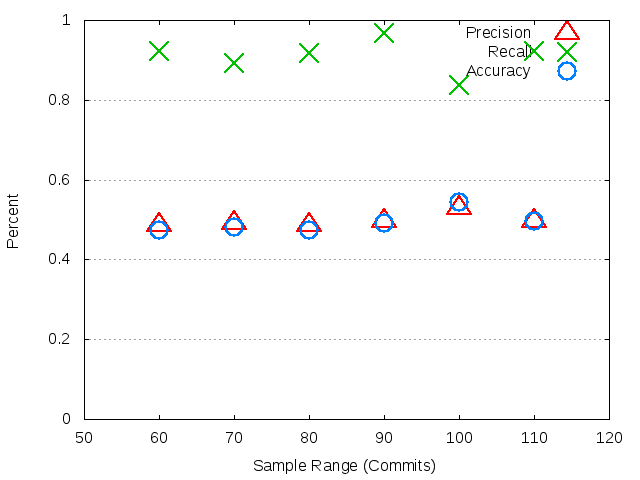
\includegraphics[width=0.8\textwidth]{images/rf/test_1/smile_sample_range.png}
\caption{\gls{swr} for smile using \gls{rf}}
\label{fig:test_1_smile_rf}
\end{figure}

% Figure for Feature Importance \gls{swr} for smile using \gls{rf}
\begin{figure}[!t]
\centering
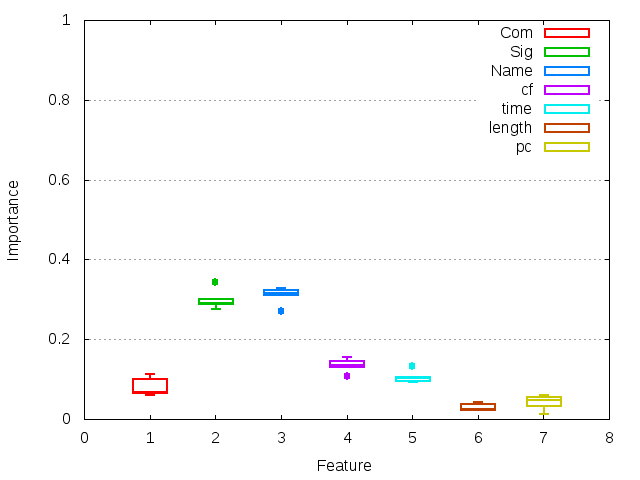
\includegraphics[width=0.8\textwidth]{images/rf/test_1/smile_importance.png}
\caption{Feature Importance \gls{swr} for smile using \gls{rf}}
\label{fig:test_1_smile_rf_importance}
\end{figure}

% Figure for \gls{swr} for ShowcaseView using \gls{rf}
\begin{figure}[!t]
\centering
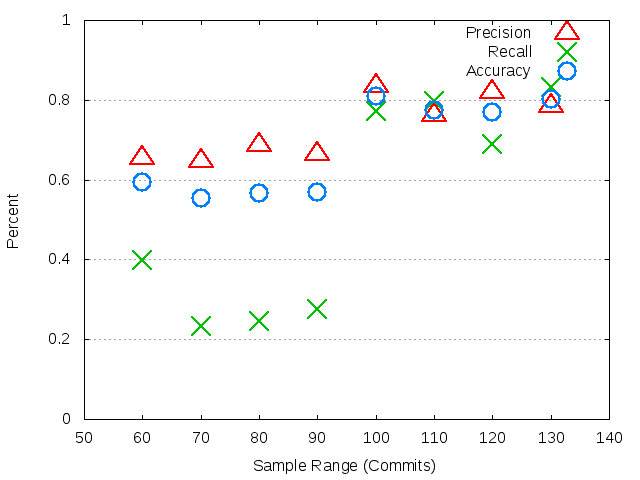
\includegraphics[width=0.8\textwidth]{images/rf/test_1/ShowcaseView_sample_range.png}
\caption{\gls{swr} for ShowcaseView using \gls{rf}}
\label{fig:test_1_ShowcaseView_rf}
\end{figure}

% Figure for Feature Importance \gls{swr} for ShowcaseView using \gls{rf}
\begin{figure}[!t]
\centering
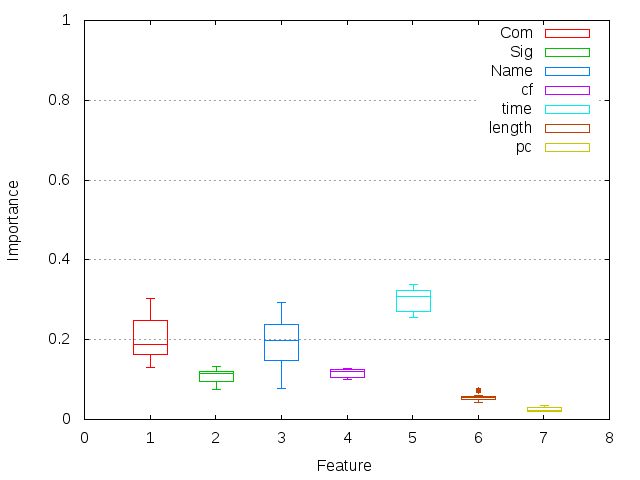
\includegraphics[width=0.8\textwidth]{images/rf/test_1/ShowcaseView_importance.png}
\caption{Feature Importance \gls{swr} for ShowcaseView using \gls{rf}}
\label{fig:test_1_ShowcaseView_rf_importance}
\end{figure}

% Figure for \gls{swr} for tempto using \gls{rf}
\begin{figure}[!t]
\centering
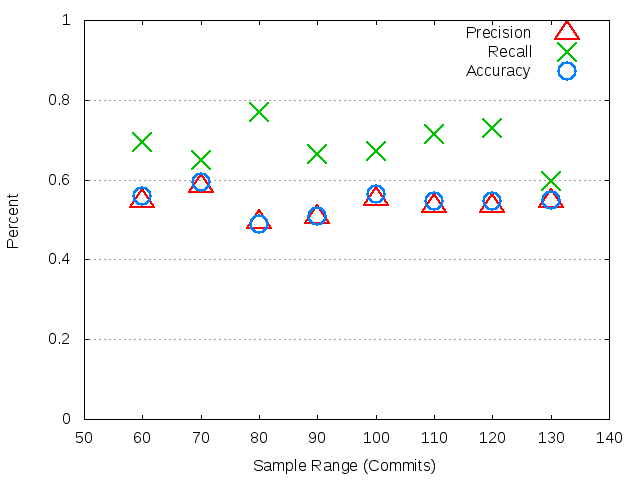
\includegraphics[width=0.8\textwidth]{images/rf/test_1/tempto_sample_range.png}
\caption{\gls{swr} for tempto using \gls{rf}}
\label{fig:test_1_tempto_rf}
\end{figure}

% Figure for Feature Importance \gls{swr} for tempto using \gls{rf}
\begin{figure}[!t]
\centering
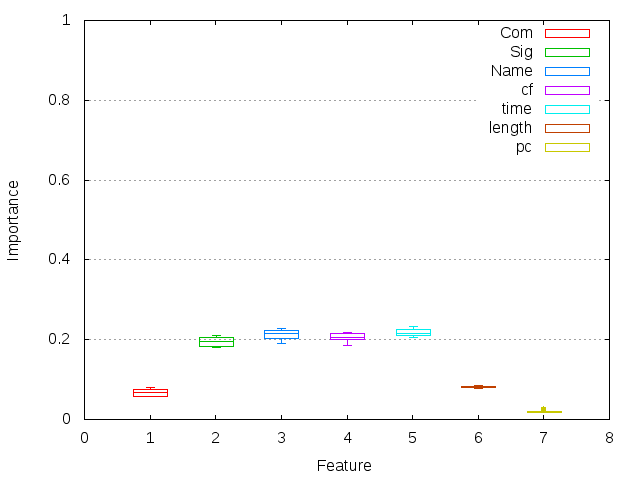
\includegraphics[width=0.8\textwidth]{images/rf/test_1/tempto_importance.png}
\caption{Feature Importance \gls{swr} for tempto using \gls{rf}}
\label{fig:test_1_tempto_rf_importance}
\end{figure}

% Figure for \gls{swr} for retrolambda using \gls{rf}
\begin{figure}[!t]
\centering
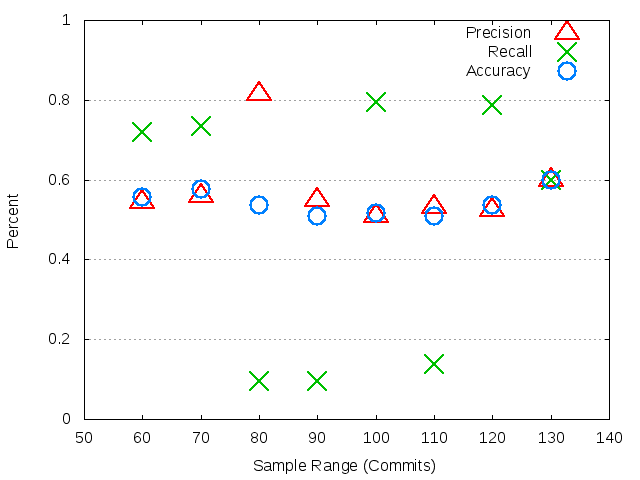
\includegraphics[width=0.8\textwidth]{images/rf/test_1/retrolambda_sample_range.png}
\caption{\gls{swr} for retrolambda using \gls{rf}}
\label{fig:test_1_retrolambda_rf}
\end{figure}

% Figure for Feature Importance \gls{swr} for retrolambda using \gls{rf}
\begin{figure}[!t]
\centering
\includegraphics[width=0.8\textwidth]{images/rf/test_1/retrolambda_importance.png}
\caption{Feature Importance \gls{swr} for retrolambda using \gls{rf}}
\label{fig:test_1_retrolambda_rf_importance}
\end{figure}

% Figure for \gls{swr} for blockly-android using \gls{rf}
\begin{figure}[!t]
\centering
\includegraphics[width=0.8\textwidth]{images/rf/test_1/blockly-android_sample_range.png}
\caption{\gls{swr} for blockly-android using \gls{rf}}
\label{fig:test_1_blockly-android_rf}
\end{figure}

% Figure for Feature Importance \gls{swr} for blockly-android using \gls{rf}
\begin{figure}[!t]
\centering
\includegraphics[width=0.8\textwidth]{images/rf/test_1/blockly-android_importance.png}
\caption{Feature Importance \gls{swr} for blockly-android using \gls{rf}}
\label{fig:test_1_blockly-android_rf_importance}
\end{figure}

% Figure for \gls{swr} for ion using \gls{rf}
\begin{figure}[!t]
\centering
\includegraphics[width=0.8\textwidth]{images/rf/test_1/ion_sample_range.png}
\caption{\gls{swr} for ion using \gls{rf}}
\label{fig:test_1_ion_rf}
\end{figure}

% Figure for Feature Importance \gls{swr} for ion using \gls{rf}
\begin{figure}[!t]
\centering
\includegraphics[width=0.8\textwidth]{images/rf/test_1/ion_importance.png}
\caption{Feature Importance \gls{swr} for ion using \gls{rf}}
\label{fig:test_1_ion_rf_importance}
\end{figure}

% Figure for \gls{swr} for brave using \gls{rf}
\begin{figure}[!t]
\centering
\includegraphics[width=0.8\textwidth]{images/rf/test_1/brave_sample_range.png}
\caption{\gls{swr} for brave using \gls{rf}}
\label{fig:test_1_brave_rf}
\end{figure}

% Figure for Feature Importance \gls{swr} for brave using \gls{rf}
\begin{figure}[!t]
\centering
\includegraphics[width=0.8\textwidth]{images/rf/test_1/brave_importance.png}
\caption{Feature Importance \gls{swr} for brave using \gls{rf}}
\label{fig:test_1_brave_rf_importance}
\end{figure}

% Figure for \gls{swr} for dagger using \gls{rf}
\begin{figure}[!t]
\centering
\includegraphics[width=0.8\textwidth]{images/rf/test_1/dagger_sample_range.png}
\caption{\gls{swr} for dagger using \gls{rf}}
\label{fig:test_1_dagger_rf}
\end{figure}

% Figure for \gls{swr} for parceler using \gls{rf}
\begin{figure}[!t]
\centering
\includegraphics[width=0.8\textwidth]{images/rf/test_1/parceler_sample_range.png}
\caption{\gls{swr} for parceler using \gls{rf}}
\label{fig:test_1_parceler_rf}
\end{figure}

% Figure for Feature Importance \gls{swr} for parceler using \gls{rf}
\begin{figure}[!t]
\centering
\includegraphics[width=0.8\textwidth]{images/rf/test_1/parceler_importance.png}
\caption{Feature Importance \gls{swr} for parceler using \gls{rf}}
\label{fig:test_1_parceler_rf_importance}
\end{figure}

\clearpage
% Figure for \gls{swr} for spark using \gls{rf}
\begin{figure}[!t]
\centering
\includegraphics[width=0.8\textwidth]{images/rf/test_1/spark_sample_range.png}
\caption{\gls{swr} for spark using \gls{rf}}
\label{fig:test_1_spark_rf}
\end{figure}

% Figure for Feature Importance \gls{swr} for spark using \gls{rf}
\begin{figure}[!t]
\centering
\includegraphics[width=0.8\textwidth]{images/rf/test_1/spark_importance.png}
\caption{Feature Importance \gls{swr} for spark using \gls{rf}}
\label{fig:test_1_spark_rf_importance}
\end{figure}

% Figure for \gls{swr} for http-request using \gls{rf}
\begin{figure}[!t]
\centering
\includegraphics[width=0.8\textwidth]{images/rf/test_1/http-request_sample_range.png}
\caption{\gls{swr} for http-request using \gls{rf}}
\label{fig:test_1_http-request_rf}
\end{figure}

% Figure for Feature Importance \gls{swr} for http-request using \gls{rf}
\begin{figure}[!t]
\centering
\includegraphics[width=0.8\textwidth]{images/rf/test_1/http-request_importance.png}
\caption{Feature Importance \gls{swr} for http-request using \gls{rf}}
\label{fig:test_1_http-request_rf_importance}
\end{figure}

\section{Experiment 2}
\label{app_sec:experiment_2}

\subsection{Support Vector Machine}
\label{app_sub:experiment_2_svm}
% params: test_3, svm

% Figure for Feature for acra using \gls{svm}
\begin{figure}
\centering
\includegraphics[width=0.8\textwidth]{images/svm/test_3/acra_sample_range.png}
\caption{Feature for acra using \gls{svm}}
\label{fig:test_3_acra_svm}
\end{figure}

% Figure for Feature for yardstick using \gls{svm}
\begin{figure}
\centering
\includegraphics[width=0.8\textwidth]{images/svm/test_3/yardstick_sample_range.png}
\caption{Feature for yardstick using \gls{svm}}
\label{fig:test_3_yardstick_svm}
\end{figure}

\clearpage

% Figure for Feature for cardslib using \gls{svm}
\begin{figure}[!t]
\centering
\includegraphics[width=0.8\textwidth]{images/svm/test_3/cardslib_sample_range.png}
\caption{Feature for cardslib using \gls{svm}}
\label{fig:test_3_cardslib_svm}
\end{figure}

% Figure for Feature for greenDAO using \gls{svm}
\begin{figure}[!t]
\centering
\includegraphics[width=0.8\textwidth]{images/svm/test_3/greenDAO_sample_range.png}
\caption{Feature for greenDAO using \gls{svm}}
\label{fig:test_3_greenDAO_svm}
\end{figure}

% Figure for Feature for mapstruct using \gls{svm}
\begin{figure}[!t]
\centering
\includegraphics[width=0.8\textwidth]{images/svm/test_3/mapstruct_sample_range.png}
\caption{Feature for mapstruct using \gls{svm}}
\label{fig:test_3_mapstruct_svm}
\end{figure}

% Figure for Feature for deeplearning4j using \gls{svm}
\begin{figure}[!t]
\centering
\includegraphics[width=0.8\textwidth]{images/svm/test_3/deeplearning4j_sample_range.png}
\caption{Feature for deeplearning4j using \gls{svm}}
\label{fig:test_3_deeplearning4j_svm}
\end{figure}

% Figure for Feature for governator using \gls{svm}
\begin{figure}[!t]
\centering
\includegraphics[width=0.8\textwidth]{images/svm/test_3/governator_sample_range.png}
\caption{Feature for governator using \gls{svm}}
\label{fig:test_3_governator_svm}
\end{figure}

% Figure for Feature for arquillian-core using \gls{svm}
\begin{figure}[!t]
\centering
\includegraphics[width=0.8\textwidth]{images/svm/test_3/arquillian-core_sample_range.png}
\caption{Feature for arquillian-core using \gls{svm}}
\label{fig:test_3_arquillian-core_svm}
\end{figure}

% Figure for Feature for fresco using \gls{svm}
\begin{figure}[!t]
\centering
\includegraphics[width=0.8\textwidth]{images/svm/test_3/fresco_sample_range.png}
\caption{Feature for fresco using \gls{svm}}
\label{fig:test_3_fresco_svm}
\end{figure}

% Figure for Feature for jadx using \gls{svm}
\begin{figure}[!t]
\centering
\includegraphics[width=0.8\textwidth]{images/svm/test_3/jadx_sample_range.png}
\caption{Feature for jadx using \gls{svm}}
\label{fig:test_3_jadx_svm}
\end{figure}

% Figure for Feature for nettosphere using \gls{svm}
\begin{figure}[!t]
\centering
\includegraphics[width=0.8\textwidth]{images/svm/test_3/nettosphere_sample_range.png}
\caption{Feature for nettosphere using \gls{svm}}
\label{fig:test_3_nettosphere_svm}
\end{figure}

\clearpage
% Figure for Feature for storm using \gls{svm}
\begin{figure}[!t]
\centering
\includegraphics[width=0.8\textwidth]{images/svm/test_3/storm_sample_range.png}
\caption{Feature for storm using \gls{svm}}
\label{fig:test_3_storm_svm}
\end{figure}

% Figure for Feature for smile using \gls{svm}
\begin{figure}[!t]
\centering
\includegraphics[width=0.8\textwidth]{images/svm/test_3/smile_sample_range.png}
\caption{Feature for smile using \gls{svm}}
\label{fig:test_3_smile_svm}
\end{figure}

% Figure for Feature for ShowcaseView using \gls{svm}
\begin{figure}[!t]
\centering
\includegraphics[width=0.8\textwidth]{images/svm/test_3/ShowcaseView_sample_range.png}
\caption{Feature for ShowcaseView using \gls{svm}}
\label{fig:test_3_ShowcaseView_svm}
\end{figure}

% Figure for Feature for tempto using \gls{svm}
\begin{figure}[!t]
\centering
\includegraphics[width=0.8\textwidth]{images/svm/test_3/tempto_sample_range.png}
\caption{Feature for tempto using \gls{svm}}
\label{fig:test_3_tempto_svm}
\end{figure}

% Figure for Feature for retrolambda using \gls{svm}
\begin{figure}[!t]
\centering
\includegraphics[width=0.8\textwidth]{images/svm/test_3/retrolambda_sample_range.png}
\caption{Feature for retrolambda using \gls{svm}}
\label{fig:test_3_retrolambda_svm}
\end{figure}

% Figure for Feature for blockly-android using \gls{svm}
\begin{figure}[!t]
\centering
\includegraphics[width=0.8\textwidth]{images/svm/test_3/blockly-android_sample_range.png}
\caption{Feature for blockly-android using \gls{svm}}
\label{fig:test_3_blockly-android_svm}
\end{figure}

% Figure for Feature for ion using \gls{svm}
\begin{figure}[!t]
\centering
\includegraphics[width=0.8\textwidth]{images/svm/test_3/ion_sample_range.png}
\caption{Feature for ion using \gls{svm}}
\label{fig:test_3_ion_svm}
\end{figure}

% Figure for Feature for brave using \gls{svm}
\begin{figure}[!t]
\centering
\includegraphics[width=0.8\textwidth]{images/svm/test_3/brave_sample_range.png}
\caption{Feature for brave using \gls{svm}}
\label{fig:test_3_brave_svm}
\end{figure}

% Figure for Feature for dagger using \gls{svm}
\begin{figure}[!t]
\centering
\includegraphics[width=0.8\textwidth]{images/svm/test_3/dagger_sample_range.png}
\caption{Feature for dagger using \gls{svm}}
\label{fig:test_3_dagger_svm}
\end{figure}

% Figure for Feature for parceler using \gls{svm}
\begin{figure}[!t]
\centering
\includegraphics[width=0.8\textwidth]{images/svm/test_3/parceler_sample_range.png}
\caption{Feature for parceler using \gls{svm}}
\label{fig:test_3_parceler_svm}
\end{figure}

\clearpage
% Figure for Feature for spark using \gls{svm}
\begin{figure}[!t]
\centering
\includegraphics[width=0.8\textwidth]{images/svm/test_3/spark_sample_range.png}
\caption{Feature for spark using \gls{svm}}
\label{fig:test_3_spark_svm}
\end{figure}

% Figure for Feature for http-request using \gls{svm}
\begin{figure}[!t]
\centering
\includegraphics[width=0.8\textwidth]{images/svm/test_3/http-request_sample_range.png}
\caption{Feature for http-request using \gls{svm}}
\label{fig:test_3_http-request_svm}
\end{figure}

\subsection{Random Forest}
\label{app_sub:experiment_2_rf}
% params: test_3, rf

% Figure for Feature for acra using \gls{rf}
\begin{figure}
\centering
\includegraphics[width=0.8\textwidth]{images/rf/test_3/acra_sample_range.png}
\caption{Feature for acra using \gls{rf}}
\label{fig:test_3_acra_rf}
\end{figure}

% Figure for Feature for yardstick using \gls{rf}
\begin{figure}
\centering
\includegraphics[width=0.8\textwidth]{images/rf/test_3/yardstick_sample_range.png}
\caption{Feature for yardstick using \gls{rf}}
\label{fig:test_3_yardstick_rf}
\end{figure}

\clearpage

% Figure for Feature for cardslib using \gls{rf}
\begin{figure}[!t]
\centering
\includegraphics[width=0.8\textwidth]{images/rf/test_3/cardslib_sample_range.png}
\caption{Feature for cardslib using \gls{rf}}
\label{fig:test_3_cardslib_rf}
\end{figure}

% Figure for Feature for greenDAO using \gls{rf}
\begin{figure}[!t]
\centering
\includegraphics[width=0.8\textwidth]{images/rf/test_3/greenDAO_sample_range.png}
\caption{Feature for greenDAO using \gls{rf}}
\label{fig:test_3_greenDAO_rf}
\end{figure}

% Figure for Feature for mapstruct using \gls{rf}
\begin{figure}[!t]
\centering
\includegraphics[width=0.8\textwidth]{images/rf/test_3/mapstruct_sample_range.png}
\caption{Feature for mapstruct using \gls{rf}}
\label{fig:test_3_mapstruct_rf}
\end{figure}

% Figure for Feature for deeplearning4j using \gls{rf}
\begin{figure}[!t]
\centering
\includegraphics[width=0.8\textwidth]{images/rf/test_3/deeplearning4j_sample_range.png}
\caption{Feature for deeplearning4j using \gls{rf}}
\label{fig:test_3_deeplearning4j_rf}
\end{figure}

% Figure for Feature for governator using \gls{rf}
\begin{figure}[!t]
\centering
\includegraphics[width=0.8\textwidth]{images/rf/test_3/governator_sample_range.png}
\caption{Feature for governator using \gls{rf}}
\label{fig:test_3_governator_rf}
\end{figure}

% Figure for Feature for arquillian-core using \gls{rf}
\begin{figure}[!t]
\centering
\includegraphics[width=0.8\textwidth]{images/rf/test_3/arquillian-core_sample_range.png}
\caption{Feature for arquillian-core using \gls{rf}}
\label{fig:test_3_arquillian-core_rf}
\end{figure}

% Figure for Feature for fresco using \gls{rf}
\begin{figure}[!t]
\centering
\includegraphics[width=0.8\textwidth]{images/rf/test_3/fresco_sample_range.png}
\caption{Feature for fresco using \gls{rf}}
\label{fig:test_3_fresco_rf}
\end{figure}

% Figure for Feature for jadx using \gls{rf}
\begin{figure}[!t]
\centering
\includegraphics[width=0.8\textwidth]{images/rf/test_3/jadx_sample_range.png}
\caption{Feature for jadx using \gls{rf}}
\label{fig:test_3_jadx_rf}
\end{figure}

% Figure for Feature for nettosphere using \gls{rf}
\begin{figure}[!t]
\centering
\includegraphics[width=0.8\textwidth]{images/rf/test_3/nettosphere_sample_range.png}
\caption{Feature for nettosphere using \gls{rf}}
\label{fig:test_3_nettosphere_rf}
\end{figure}

\clearpage
% Figure for Feature for storm using \gls{rf}
\begin{figure}[!t]
\centering
\includegraphics[width=0.8\textwidth]{images/rf/test_3/storm_sample_range.png}
\caption{Feature for storm using \gls{rf}}
\label{fig:test_3_storm_rf}
\end{figure}

% Figure for Feature for smile using \gls{rf}
\begin{figure}[!t]
\centering
\includegraphics[width=0.8\textwidth]{images/rf/test_3/smile_sample_range.png}
\caption{Feature for smile using \gls{rf}}
\label{fig:test_3_smile_rf}
\end{figure}

% Figure for Feature for ShowcaseView using \gls{rf}
\begin{figure}[!t]
\centering
\includegraphics[width=0.8\textwidth]{images/rf/test_3/ShowcaseView_sample_range.png}
\caption{Feature for ShowcaseView using \gls{rf}}
\label{fig:test_3_ShowcaseView_rf}
\end{figure}

% Figure for Feature for tempto using \gls{rf}
\begin{figure}[!t]
\centering
\includegraphics[width=0.8\textwidth]{images/rf/test_3/tempto_sample_range.png}
\caption{Feature for tempto using \gls{rf}}
\label{fig:test_3_tempto_rf}
\end{figure}

% Figure for Feature for retrolambda using \gls{rf}
\begin{figure}[!t]
\centering
\includegraphics[width=0.8\textwidth]{images/rf/test_3/retrolambda_sample_range.png}
\caption{Feature for retrolambda using \gls{rf}}
\label{fig:test_3_retrolambda_rf}
\end{figure}

% Figure for Feature for blockly-android using \gls{rf}
\begin{figure}[!t]
\centering
\includegraphics[width=0.8\textwidth]{images/rf/test_3/blockly-android_sample_range.png}
\caption{Feature for blockly-android using \gls{rf}}
\label{fig:test_3_blockly-android_rf}
\end{figure}

% Figure for Feature for ion using \gls{rf}
\begin{figure}[!t]
\centering
\includegraphics[width=0.8\textwidth]{images/rf/test_3/ion_sample_range.png}
\caption{Feature for ion using \gls{rf}}
\label{fig:test_3_ion_rf}
\end{figure}

% Figure for Feature for brave using \gls{rf}
\begin{figure}[!t]
\centering
\includegraphics[width=0.8\textwidth]{images/rf/test_3/brave_sample_range.png}
\caption{Feature for brave using \gls{rf}}
\label{fig:test_3_brave_rf}
\end{figure}

% Figure for Feature for dagger using \gls{rf}
\begin{figure}[!t]
\centering
\includegraphics[width=0.8\textwidth]{images/rf/test_3/dagger_sample_range.png}
\caption{Feature for dagger using \gls{rf}}
\label{fig:test_3_dagger_rf}
\end{figure}

% Figure for Feature for parceler using \gls{rf}
\begin{figure}[!t]
\centering
\includegraphics[width=0.8\textwidth]{images/rf/test_3/parceler_sample_range.png}
\caption{Feature for parceler using \gls{rf}}
\label{fig:test_3_parceler_rf}
\end{figure}

\clearpage
% Figure for Feature for spark using \gls{rf}
\begin{figure}[!t]
\centering
\includegraphics[width=0.8\textwidth]{images/rf/test_3/spark_sample_range.png}
\caption{Feature for spark using \gls{rf}}
\label{fig:test_3_spark_rf}
\end{figure}

% Figure for Feature for http-request using \gls{rf}
\begin{figure}[!t]
\centering
\includegraphics[width=0.8\textwidth]{images/rf/test_3/http-request_sample_range.png}
\caption{Feature for http-request using \gls{rf}}
\label{fig:test_3_http-request_rf}
\end{figure}

